\section{\secsubsets}
\label{sec_subsets}

We continue our discussion of sets by revisiting the concept of a subset and describing how to represent subsets using bit strings. Next, we consider sets whose elements are also sets, including the set of all subsets of a set.  We conclude by working with set-theoretic functions.

%%%%%%%%%%%%%%%%%%%%%%%%

\newcommand{\subsubsets}{Subsets of a Set}
\subsection{\subsubsets}
\label{sub_subsets}

We first encountered subsets in \Cref{sec_counting_subsets}.  We repeat that initial description here.  In many situations, we want to select some of the elements of a set.  We can think of a set as corralling its elements inside a rope.  For example, the set $A=\{1,2,3,7,8\}$ is drawn in \Cref{fig_subset_corral_again}.  If we corral some, all, or none of the elements within $A$, we get a subset of $A$.  For example, \Cref{fig_subset_corral_again} shows the subset $\{2,8\}$ shaded in gray.

\begin{figure}[ht]
    \centering
        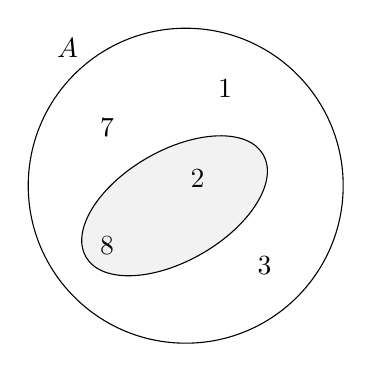
\begin{tikzpicture}[set/.style={fill=gray,fill opacity=0.1}]
            \scope
            \clip 
            (0,0) circle (1);
            \endscope
    \draw (0,0) circle (2) 
        (-1.5,1.5) node [text=black,above] {$A$}
          (.5,1)node [text=black,above] {$1$}
            (.15,-.15)node [text=black,above] {$2$}
              (1,-1.25)node [text=black,above] {$3$}
                (-1,.5)node [text=black,above] {$7$}
                  (-1,-1)node [text=black,above] {$8$}
                      %(1,.5) node [text=black,above] {$B$}
    ;
    \draw[set,rotate =30] (-.25,-.15) ellipse (1.3cm and .7cm);
    \end{tikzpicture}
    \caption{The subset $\{2,8\}$ corrals some of the elements of the set $A=\{1,2,3,7,8\}$.}
        \label{fig_subset_corral_again}
\end{figure}

We state a more formal definition of a subset.

\begin{defn}[Subsets (formal)]
\label{defn_subsets_formal}
~
    \begin{apart}
        \item The set $S$ is a \vocab{subset} of the set $A$, denoted $S \subseteq A$, if every element of $S$ is an element of $A$. That is, $\forall x \in S, x \in A$ or, equivalently,
        $$x \in S \to x \in A.$$  For example, $\{2,8\} \subseteq \{1,2,3,7,8\}$ because $2 \in \{1,2,3,7,8\}$ and $8 \in \{1,2,3,7,8\} $. Similarly, $\{3\} \subseteq \{1,2,3,7,8\}$ because $3 \in \{1,2,3,7,8\}$. Note that $\{3\}$ is different from the integer 3. For example, it would not be appropriate to write $3 \subseteq \{1,2,3,7,8\}$ without the set brackets around 3.
        
        \item If the set $S$ is not a subset of the set $A$, we write $S \nsubseteq A$.  For example, $\{1,5,6\}\nsubseteq \{1,2,3,7,8\}$ because, for example, $5 \in \{1,5,6\}$ but $5 \notin \{1,2,3,7,8\}$.

        \item Note that the set $A$ is a subset of itself.  Think of corralling all the elements of $A$.  For example, $\{1,2,3,7,8\} \subseteq \{1,2,3,7,8\}$. A subset $S$ of a set $A$ is \vocab{proper} if $S \neq A$.  For example $\{2,8\}$ is a proper subset of $\{1,2,3,7,8\}$. 
    \end{apart}
\end{defn}

We note that the empty set is a subset of any set.

\begin{rem}[Empty set is subset of any set]
\label{rem_empty_set_is_subset}
    The empty set $\varnothing$ is a subset of any set.
\end{rem}

For example, $\varnothing \subseteq \{1,2,3,7,8\}$.  Think of corralling no elements of $A$ or drawing a shaded shape within $A$ that contains none of the elements of $A$. Note that any statement beginning $\forall x \in \varnothing$ is vacuously true since there is nothing to check.  In particular, $\forall x \in \varnothing, x \in A$ is true.  Similarly, any statement beginning ``if $x \in \varnothing$'' is also true because $x \in \varnothing$ is false and any conditional with false hypothesis is true.  In particular, $x \in \varnothing \to x \in A$ is true. 

Let's look at another example of subsets.

\begin{exam}[Subsets]
\label{exam_subsets}
~
    \begin{apart}
        \item List all subsets of $\{1,2,3,4\}$.
            \begin{soln}
                Let's organize our list by the number of elements in the subset, as in \Cref{table_subsets_1234}.  There are 16 subsets listed.

                \begin{table}[hbtp]
                    \centering
                    \begin{tabular}{ll}
                         0 elements: & $\varnothing$ \\
                         1 element: & $\{1\}, \{2\},\{3\},\{4\}$ \\
                         2 elements: & $\{1,2\}, \{1,3\},\{1,4\},\{2,3\},\{2,4\},\{3,4\}$ \\
                         3 elements: & $\{1,2,3\}, \{1,2,4\},\{1,3,4\},\{2,3,4\}$ \\
                         4 elements: & $\{1,2,3,4\}$
                    \end{tabular}
                    \caption{The subsets of $\{1,2,3,4\}$.}
                    \label{table_subsets_1234}
                \end{table}
            \end{soln}
        \item How many 3-element subsets does $A = \{1,2,3,4,5\}$ have?
            \begin{soln}
                There are $\binom{5}{3}$ 3-element subsets from a set of 5 elements, by definition of the binomial coefficients (\Cref{defn_binomial_coeff}).  We can evaluate $\binom{5}{3}=10$, or just leave the answer as $\binom{5}{3}$.
            \end{soln}
        \item \label{part_number_subsets} How many subsets does $A = \{1,2,3,4,5\}$ have?
            \begin{soln}
                The phrase ``how many'' indicates that we are counting.  Let's think about how to select a subset $S$ of $A$.  Step 1: decide if $1 \in S$.  There are 2 choices: yes or no. (2 ways)  Step 2: decide if $2 \in S$.  There are again 2 choices: yes or no. (2 ways) Step 3: decide if $3 \in S$. (2 ways). Step 4: decide if $4 \in S$. (2 ways).  Step 5: decide if $5 \in S$. (2 ways). Since steps multiply (\Cref{thm_steps_multiply}), there are $2\cdot 2 \cdot 2 \cdot 2 \cdot 2 = 2^5$ subsets.

                % Note that we could alternatively have counted the number of subsets of each possible size to get
                %     $$\binom{5}{0}+\binom{5}{1}+\binom{5}{2}+\binom{5}{3}+\binom{5}{4}+\binom{5}{5} = 1+5+10+10+5+1 =32 = 2^5,$$
                % where we could evaluate the binomial coefficients using the arithmetic triangle as in \Cref{figure_arith_tri_standard}.
            \end{soln}
    \end{apart}
\end{exam}

The result of \Cref{exam_subsets} (\ref{part_number_subsets}) holds in general

\begin{thm}[Number of subsets]
\label{thm_number_subsets} 
    A set with $n$ elements has $2^n$ subsets.
\end{thm}

Let's look at an infinite example.

\begin{exam}[Multiples of six are subset of evens]
\label{exam_mult6_subset_evens}
    Consider the sets 
        $$E=\{2k \mid k \in \mathbb{N}\}$$
    and 
        $$X = \{6k \mid k \in \mathbb{N}\}.$$
        \begin{apart}
            \item Write $E$ and $X$ using a list and $\ldots$ notation.
                \begin{soln}
                    We can write $E = \{0,2,4,6, \ldots\}$ and $X = \{0,6,12,18,\ldots\}$.
                \end{soln}
            \item \label{part_subset_proof} Prove that $X$ is a subset of $E$.
                \begin{soln}
                    We need to prove: if $n \in X$, then $n \in E$.  We use a direct proof of the conditional (\Cref{pff_if_then_direct}).

                    \emph{Proof} Let $n \in X$. By definition of $X$ we can write $n = 6k$ for some $k \in \mathbb{N}$.  Note that $$n = 6k=2(3k)$$
                    and so $n = 2k'$ where $k'=3k \in \mathbb{N}$.  Therefore, by definition of $X$, it follows that $n \in E$.
                \end{soln}
            \item Prove that $X$ is a proper subset of $E$.
                \begin{soln}
                    Since we know that $X$ is a subset, it remains to show that $X$ is proper.  For that, all we need is an example of $E-X$, that is, an element of $E$ that is not in $X$.  Any even number that is not a multiple of 6 will do.  For example, $4 \in E$ but $4 \notin X$.
                \end{soln}
        \end{apart}
\end{exam}

We can use the idea of subsets to show that two sets are equal.

\begin{exam}[Proof two sets are equal]
\label{exam_proof_sets_equal}    
    Let $S = \{ b \in \mathbb{B}_5 \mid b \text{ has exactly two \bs{0}s } \}$ and let $T = \{ b \in \mathbb{B}_5 \mid b \text{ has exactly three \bs{1}s } \}$ where $\mathbb{B}_5$ is the set of bit strings of length five.  For example, $\bs{10101} \in S$ because it has two \bs{0}s and $\bs{10101} \in T$ because it has three \bs{1}s. Can you see that $S = T$?  Prove $S=T$. 
        \begin{soln}
            \emph{Proof:} First, let $b \in S$.  That is, $b$ is a bit string of length five that has exactly two \bs{0}s.  The remaining $5-2=3$ bits must be \bs{1}s. Thus $b \in T$.  
            
            Conversely, let $b \in T$.  That is, $b$ is a bit string of length five that has exactly three \bs{1}s.  The remaining $5-3=2$ bits must be \bs{0}s.  Thus $b \in S$.
        \end{soln}
\end{exam}

Notice in \Cref{exam_proof_sets_equal} that we showed $S=T$ by showing that $S \subseteq T$ (if $x \in S$, then $x \in T$) and then showing the converse that $T \subseteq S$ (if $x \in T$, then $x \in S$), as in \Cref{defn_converse}.
Putting these two parts together, we conclude that the elements of $S$ and $T$ are the same, and so $S=T$.

It is your turn to work with subsets.

\begin{act}[Subsets]
\label{act_subsets}
~
    \begin{actpart}
        \item Check that $T=\{2,5\} \subseteq S=\{1,2,3,4,5,6\}$.
        \item Show that $V = \{2,8\} \not \subseteq S=\{1,2,3,4,5,6\}$.
        \item List all subsets of $\{1,2,3\}$. 
        \item \label{part_number_subsets_n} How many subsets does $\{1,2,3,\ldots,n\}$ have? Hint: Count using Step 1: Decide if 1 is in the subset (yes/no). Step 2: Decide if 2 is in the subset (yes/no). And so on.
        \item Consider the sets $Q = \{ n^2 \mid n \in \mathbb{N}\}$ and $P = \{2^n \mid n \in \mathbb{N}\}$.  Describe $Q$ and $P$ in words, then show that neither of $Q$ or $P$ is a subset of the other.
        \item If the set $S$ is a subset of the set $A$, then explain how to simplify $S \cap A$ and $S \cup A$.
    \end{actpart}
\end{act}

%%%%%%%%%%%%%%%%%%%%%%%%

\newcommand{\subbsrepsubset}{Bit String Representation of Subsets}
\subsection{\subbsrepsubset}
\label{sub_bs_rep_subset}

Set operations can be useful in sorting data, as we saw in the examples in \Cref{defn_set_ops}.  But working with sets can be bulky. It turns out that we can represent subsets using bit strings, and we can encode set operations as bit string operations.

\begin{defn}[Bit string representation of subsets]
\label{defn_bs_rep_subsets}
~    
    \begin{apart}
        \item Let $U = \{a_1, a_2, a_3, \ldots, a_n\}$ be a finite set and let $S$ be a subset of $U$.  The \vocab{bit string representation} of $S$ (in $U$)  is $b=b_1b_2b_3\ldots b_n$ where 
            $$b_i = \left\{ \begin{array} {cl} \bs{1} & \text{if } a_i \in S \\ \bs{0} & \text{if } a_i \not\in S \\ \end{array} \right. $$  
        For example, for $U = \{1,2,3,4,5,6\}$, let's calculate the bit string representation of the subset $S =\{1,2,3\}$. It can help to write the universal set as a reference set as in \Cref{tab_bs_rep_subsets}.

            \begin{table}[htbp]
                \centering
                \begin{tabular}{c|cccccc}
                $U$ & 1 & 2 & 3 & 4 & 5 & 6\\ \hline
                $S$ & 1 & 2 & 3 &   &   &  \\ \hline
                $b$ & \bs{1} & \bs{1} & \bs{1} & \bs{0} & \bs{0} & \bs{0} 
                \end{tabular}
                \caption{Representing the subset $S =\{1,2,3\}$ of the universal set $U = \{1,2,3,4,5,6\}$ using the bit string $b=\bs{111000}$.}
                \label{tab_bs_rep_subsets}
            \end{table}
  
        The first bit of $b$ is \bs{1} because $1 \in S$, the second bit of $b$ is \bs{1} because $2 \in S$, the third bit of $b$ is \bs{1} because $3 \in S$, the fourth bit of $b$ is \bs{0} because $4 \notin S$, the fifth bit of $b$ is \bs{0} because $5 \notin S$, and the sixth bit of $b$ is \bs{0} because $6 \notin S$.  Thus, $b=\bs{111000}$.
        
        \item When $b=b_1b_2b_3\ldots b_n$ is the bit string representing the subset $S$ (in a universal set $U$), we write
        $$S \leftrightarrow b.$$  For example, $\{1,2,3\} \leftrightarrow \bs{111000}$.  
    \end{apart}
\end{defn}

Note that each subset of $U$ has a unique bit string and each bit string has a unique subset.  That is, $S \leftrightarrow b$ is a pairing. We can use bit-wise operators to perform set operations.  Here is an example.

\begin{exam}[The AND operator on bit strings and its connection to set operations]
\label{exam_bs_rep_AND}
    Given bit strings $b$ and $c$ each of length $n$.  Define the AND operator ($\land$) as follows:
        \begin{itemize}
            \item $\bs{0} \land \bs{0} = \bs{0}$, $\bs{0} \land \bs{1} = \bs{0}$, $\bs{1} \land \bs{0} = \bs{0}$, and $\bs{1} \land \bs{1} = \bs{1}$.  Think of \bs{0} = False and \bs{1} = True.
            \item Each bit of $b \land c$ is the $\land$ of the corresponding bit of $b$ and the corresponding bit of $c$.
        \end{itemize}

        \begin{apart}
            \item If $b = \bs{10011}$ and $c = \bs{11001}$, calculate $b \land c$.
                \begin{soln}
                    We have
                    $$b \land c = \begin{array}{cccccc} 
                    & \bs{1} & \bs{0} & \bs{0} & \bs{1} & \bs{1} \\
                    \land  & \bs{1} & \bs{1} & \bs{0} & \bs{0} & \bs{1} \\ \hline 
                    & \bs{1} & \bs{0} & \bs{0} & \bs{0} & \bs{1} \\ \end{array}$$
                    Thus $b \land c= \bs{10001}$.
                \end{soln}
            \item In the set $U = \{1,2, 3, 4, 5\}$, find the subsets corresponding to $b$, to $c$, and to $b \land c$. 
                \begin{soln}
                    We can write the universal set as a reference set to get
                        \begin{center}
                            \begin{tabular}{c|ccccc}
                                $U$ & 1 & 2 & 3 & 4 & 5 \\ \hline
                                $b$ & \bs{1} & \bs{0} & \bs{0} & \bs{1} & \bs{1} \\
                                $c$ & \bs{1} & \bs{1} & \bs{0} & \bs{0} & \bs{1} \\
                                $b \land c$ & \bs{1} & \bs{0} & \bs{0} & \bs{0} & \bs{1}
                            \end{tabular}
                        \end{center}
                    Thus $b \leftrightarrow \{1, 4, 5 \}$, $c  \leftrightarrow \{1, 2, 5\}$, and $b \land c \leftrightarrow \{1, 5\}$.
                \end{soln}
            \item Make a conjecture about the relationship in general: if $b \leftrightarrow S$ and $c \leftrightarrow T$, then $b \land c \leftrightarrow \underline{\hspace{1in}}$.
                \begin{soln}
                    Suppose $b \leftrightarrow S$ and $c \leftrightarrow T$. The only way we have a \bs{1} in $b \land c$ is when there is a \bs{1} in $b$ and a \bs{1} in the same place in $c$.  That is, when that element of $U$ is in the set $S$ and in the set $T$.  We conjecture that $$b \land c \leftrightarrow S \cap T.$$
                \end{soln}
        \end{apart}
\end{exam}

Try working with the bit string representation of subsets.

\begin{act}[Bit string representation of subsets]
\label{act_bs_rep_subsets}
~
    \begin{apart}
        \item List the bit string corresponding to each subset of $U = \{1,2,3,4,5,6,7,8,9,10\}$: 
            \begin{center}
                $\{1,3,5,7,9\}$, $\{2, 4, 6, 8, 10\}$, $\{10\}$, and $U$.
            \end{center}
            
        \item List the subset of $U = \{1,2,3,4,5,6,7,8,9,10\}$ corresponding to each bit string: 
            \begin{center}
                $\bs{1100110011}$, $\bs{1000000001}$, and $\bs{0000000000}$.
            \end{center}  
        
        \item For any set $U$, if the bit string $b$ corresponds to the subset $S$, what does the weight of $b$ tell you about $S$?

        \item \label{part_OR} Given bit strings $b$ and $c$ each of length $n$.  Define the OR operator ($\lor$) as follows:
            \begin{itemize}
                \item $\bs{0} \lor \bs{0} = \bs{0}$, $\bs{0} \lor \bs{1} = \bs{1}$, $\bs{1} \lor \bs{0} = \bs{1}$, and $\bs{1} \lor \bs{1} = \bs{1}$.  Think of \bs{0} = False and \bs{1} = True.  
                \item Each bit of $b \lor c$ is the $\lor$ of the corresponding bit of $b$ and the corresponding bit of $c$. 
            \end{itemize}
        Calculate $b \lor c$ if $b = \bs{10011}$ and $c = \bs{11001}$. It might help to line up the bit strings as follows.
            $$b \lor c = 
                \begin{array}{cccccc} 
                & \bs{1} & \bs{0} & \bs{0} & \bs{1} & \bs{1} \\
                \lor  & \bs{1} & \bs{1} & \bs{0} & \bs{0} & \bs{1} \\ \hline 
                & \underline{\hspace{.1in}} & \underline{\hspace{.1in}} & \underline{\hspace{.1in}} & \underline{\hspace{.1in}} & \underline{\hspace{.1in}}  \end{array}$$
                
        \item In the universal set $U = \{1,2, 3, 4, 5\}$, write the subsets corresponding to $b = \bs{10011}$, $c = \bs{11001}$, and $b \lor c$. It might help to write the universal set as a reference.
            \begin{center}
                \begin{tabular}{c|ccccc}
                    $U$ & 1 & 2 & 3 & 4 & 5 \\ \hline
                    $b$ & \bs{1} & \bs{0} & \bs{0} & \bs{1} & \bs{1} \\
                    $c$ & \bs{1} & \bs{1} & \bs{0} & \bs{0} & \bs{1} \\
                    $b \lor c$ & \underline{\hspace{.1in}} & \underline{\hspace{.1in}} & \underline{\hspace{.1in}} & \underline{\hspace{.1in}} & \underline{\hspace{.1in}}
                \end{tabular}
            \end{center}
        \item How is the set corresponding to $b \lor c$ related to the sets corresponding to $b$ and to $c$?  
        \item Make a conjecture about the relationship in general: if $b \leftrightarrow S$ and $c \leftrightarrow T$, then $b \lor c \leftrightarrow \underline{\hspace{1in}}$.
    \end{apart}
\end{act}

%%%%%%%%%%%%%%%%%%%%%%%%

\newcommand{\subsetsofsets}{Sets of Sets}
\subsection{\subsetsofsets}
\label{sub_sets_of_sets}

A set can contain any type of object, including sets.  For example, in \Cref{defn_ordered_pairs} we see the set $(x,y)=\{\{x\},\{x,y\}\}$.

\begin{exam}[Two-element sets]
\label{exam_2elt_sets}
    Each of the following sets has two elements: 
        $\{x, y\}$, $\{x,\{y\}\}$,$\{\{x\},\{y\}\}$, 
        and $\{\{x\}, \{x,y\} \}.$
        \begin{apart}
            \item List the elements of each set.
                \begin{soln}
                    The outermost set of brackets denote the start and end of our set.  When we remove the outermost set of brackets we get the list of elements.
                        \begin{center}
                            \begin{tabular}{l|l}
                                set & elements \\ \hline
                                $\{x, y\}$ &  $x$ and $y$\\
                                $\{x,\{y\}\}$ & $x$ and $\{y\}$ \\
                                $\{\{x\},\{y\}\}$ & $\{x\}$ and $\{y\}$ \\
                                $\{\{x\}, \{x,y\} \}$ & $\{x\}$ and $\{x,y\}$ 
                            \end{tabular}
                        \end{center}
                    Note that the presence or absence of set brackets is important. 
                \end{soln}
            \item Which of those sets contains the element $x$?  The element $y$?
                \begin{soln}
                    Looking at the list of elements, we see that the sets $\{x, y\}$ and $\{x,\{y\}\}$ contain the element $x$, but only the set $\{x, y\}$ contains the element $y$.
                \end{soln}
        \end{apart}
\end{exam}

The set of all subsets of a set has a name.

\begin{defn}[Power set]
\label{defn_power_set}
    Given a set $A$, the \vocab{power set} of $A$, denoted $\mathscr{P}(A)$ is the set of all subsets of $A$.  That is, $\mathscr{P}(A) = \{ S \mid S \subseteq A\}$.  For example, the power set of $\{0,1\}$ is $\mathscr{P}(\{0,1\}) = \{ \varnothing, \{0\}, \{1\}, \{0,1\}\}$.
\end{defn}

We can use set-builder notation to define a set of sets.

\begin{exam}[Sets of sets defined using set-builder notation]
\label{exam_set_of_sets_setbuilder}
    Give examples of two different elements in each set.  Recall that $\mathscr{P}(\mathbb{Z})$ is the set of all subsets of $\mathbb{Z}$.
        \begin{apart}
            \item $\mathscr{S} = \{ A \in \mathscr{P}(\mathbb{Z}) \mid 2 \in A \text{ but }-3 \notin A\} $
                \begin{soln}
                    We want subsets of $\mathbb{Z}$ that contain 2 but not -3.  One example is $\{2,4,6\}$ since $2 \in \{2,4,6\}$ and $-3 \notin \{2,4,6\}$.   Another example is $\mathbb{N}$ because $2 \in \mathbb{N}$ but $-3 \notin \mathbb{N}$.
                \end{soln}
            \item $\mathscr{T} = \{A \in \mathscr{P}(\mathbb{Z}) \mid |A|=3\}$
                \begin{soln}
                    We want subsets of $\mathbb{Z}$ that have three elements.  One example is $\{2,4,6\}$ and another example is $\{113, 872, 987\}$.
                \end{soln}
        \end{apart}
\end{exam}

Try working with sets of sets.

\begin{act}[Sets of sets]
\label{act_sets_of_sets}
~
    \begin{actpart}
        \item Calculate the power set $\mathscr{P}(\{1,2\})$. 
        \item Calculate the power set $\mathscr{P}(\{0,1,2\})$. 
        \item For a finite set $A$, how is $|\mathscr{P}(A)|$ related to $|A|$?
        \item List the elements of $C=\{ \{a\},b,\{\{a\},b\}\}$.  How many elements does $C$ have?
        \item For that same set $C=\{ \{a\},b,\{\{a\},b\}\}$, explain why $\{\{a\},b\} \in C$ and then explain why $\{\{a\},b\} \subseteq C$
        \item Recall that $\mathscr{P}(\mathbb{Z})$ is the set of all subsets of $\mathbb{Z}$.  Give two examples of elements of the set $\mathscr{D} = \{ A \in \mathscr{P}(\mathbb{Z}) \mid A \cap \{1,2,3\} = \varnothing\}$.
    \end{actpart}
\end{act}

%%%%%%%%%%%%%%%%%%%%%%%%

\newcommand{\subsetfn}{Detour: Set-theoretic Functions}
\subsection{\subsetfn}
\label{sub_set_functions}

In \Cref{sec_fn_words}, we saw functions that involve bit strings, number theory, and graph theory.  Let's look at some examples of functions involving set theory.

\begin{exam}[Is 7 in set?]
\label{exam_is7_function} 
    The function $\fn{seven}:\mathscr{P}(\{0,1,2,3,4,5,6,7,8,9\}) \to \{0,1\}$ is defined by 
        $$\fn{seven}(A) = \left\{
        \begin{array}{cl}
        1 & \text{ if }7 \in A \\
        0 & \text{ if }7 \notin A \\
        \end{array}
        \right.$$
        \begin{apart}
            \item Identify the domain and codomain of $\fn{seven}$.
                \begin{soln}
                    The domain of $\fn{seven}$ is $\mathscr{P}(\{0,1,2,3,4,5,6,7,8,9\})$ and the codomain of $\fn{seven}$ is $\{0,1\}$.
                \end{soln}
            \item Evaluate $\fn{seven}(\{1,3,4,7\})$ and $\fn{seven}(\{0,2,4,6,8\})$. 
                \begin{soln}
                    Since 7 is one of the elements in $\{1,3,4,7\}$, we are in the first case and so $\fn{seven}(\{1,3,4,7\})=1$. 
                    Since 7 is not one of the elements in $\{0,2,4,6,8\}$, we are in the second case and so $\fn{seven}(\{0,2,4,6,8\})=0$.
                \end{soln}
            \item Identify the image of $\fn{seven}$.
                \begin{soln}
                    The image is $\{0,1\}$ because the only outputs are 0 and 1 (and both happen).
                \end{soln}
            \item Is $\fn{seven}$ onto?  Is $\fn{seven}$ one-to-one?
                \begin{soln}
                    First, $\fn{seven}$ is onto because the image is the entire codomain.  For example, we saw that $\fn{seven}(\{0,2,4,6,8\})=0$ and $\fn{seven}(\{1,3,4,7\})=1$. 

                    Next, $\fn{seven}$ is not one-to-one because, for example, $\fn{seven}(\{0,2,4,6,8\})=0$ and $\fn{seven}(\{1,2,3,4\})=0$.
                \end{soln}
        \end{apart}
\end{exam}

Here is another example.

\begin{exam}[Cardinality of a set]
\label{exam_cardinality_fn_set}
    The function $\fn{card}:\mathscr{P}(\{0,1,2,3,4,5,6,7,8,9\}) \to \mathbb{N}$ is defined by $\fn{card}(A)=|A|$, the number of elements in the set $A$.
        \begin{apart}
            \item Evaluate $\fn{card}(\{1,4,5,7\})$ and $\fn{card}(\{0\})$.
                \begin{soln}
                    The set $\{1,4,5,7\}$ has four elements, so $\fn{card}(\{1,4,5,7\})=4$.  The set $\{0\}$ has one element, so $\fn{card}(\{0\})=1$.
                \end{soln}
            \item Identify the domain, codomain, and image of $\fn{card}$.
                \begin{soln}
                    The domain is $\mathscr{P}(\{0,1,2,3,4,5,6,7,8,9\})$, meaning we can input any subset of $\{0,1,2,3,4,5,6,7,8,9\}$. The codomain is $\mathbb{N}$ meaning the output is always a nonnegative integer.  The image is the set of actual output values.  Since each subset of $\{0,1,2,3,4,5,6,7,8,9\}$ has between 0 and 10 elements, and all are possible, the image is $\{0,1,2,3,4,5,6,7,8,9,10\}$.
                \end{soln}
            \item How many elements $A$ of $\mathscr{P}$ have $\fn{card}(A)=4$?  Explain how you counted.
                \begin{soln}
                    A set $A$ has $\fn{card}(A)=4$ exactly when $A$ has four elements.  The number of 4-element subsets of $\{0,1,2,3,4,5,6,7,8,9\}$ is, by \Cref{defn_binomial_coeff}, exactly $\binom{10}{4}$.  (If you are curious, $\binom{10}{4}=210$.
                \end{soln}
            \item Is $\fn{card}$ onto?  Is $\fn{card}$ one-to-one?
                \begin{soln}
                    First, $\fn{card}$ is not onto because, for example, $\fn{card}(A)=11$ is impossible because $A$ can have at most 10 elements.

                    Next, $\fn{card}$ is not one-to-one. We just saw that there are 210 sets $A$ with $\fn{card}(A) = 4$.
                \end{soln}
        \end{apart}    
\end{exam}

Now it is your turn to work with functions that involve sets.

\begin{act}[Set-theoretic functions]
\label{act_set_fns}
    Let $P = \mathscr{P}(\mathbb{N})$, the set of all subsets of $\mathbb{N}$, and let $P^*$ be the set of all nonempty subsets of $\mathbb{N}$.
    \begin{apart}
        \item The function $\fn{del7}: P \to P$ is defined by $\fn{del7}(A) = A-\{7\}$.  Evaluate $\fn{del7}(\{2,4,7\})$ and $\fn{del7}(\{1,2,3,4\})$.  What are the fixed points of $\fn{del7}$, meaning which sets $A$ have $\fn{del7}(A) = A$?
        \item The function $\fn{max}:P^* \to \mathbb{N}$ is defined by $\fn{max}(A)=$ the largest integer in $A$.  Evaluate $\fn{max}(\{2,4,7\})$.  How many sets $A$ have $\fn{max}=2$?  List them.
        \item Give counterexamples to show that $\fn{del7}$ and $\fn{max}$ are not one-to-one.
        \item Give a counterexample to show that $\fn{del7}$ is not onto.
        \item Prove that $\fn{max}$ is onto.
    \end{apart}
\end{act}

%%%%%%%%%%%%%%%%%%%%%%%%%%%%%%%%%%%
\subsection{Exercises}

%%%%%%%%%%%%%%%%%%%%%%%%

\subsubsection*{Exercises for \Cref{sub_subsets}
\subsubsets}

\begin{exer}[\exerP] % subsets notation]
\label{exer_subset_notation}
    Consider $S = \{0, 2, 4\}$, $T = \{1, 2, 3\}$, $V = \{2\}$, and $E = \{ n \in \mathbb{Z} \mid n \text{ is even} \}$.
        \begin{exerpart}
            \item Explain why $T \not\subseteq S$.
            \item Explain why $V \subseteq S \cap T$.
            \item Is $S \subseteq E$? Explain.
        \end{exerpart}
\end{exer}

\begin{exer}[\exerP] % subsets of bit strings]
\label{exer_subset_bs}
    Consider the set of bit strings $B = \{00, 01, 11\}$.
        \begin{exerpart}
            \item List all elements of $B$ and determine $|B|$.
            \item List all subset of $B$ and count the number of subsets of $B$.
        \end{exerpart}
\end{exer}

\begin{exer}[\exerP] % squares and powers of 2 subsets]
\label{exer_squares_powers2_subsets}
    Consider the sets $Q = \{ n^2 \mid n \in \mathbb{N}\}$ and $P = \{2^n \mid n \in \mathbb{N}\}$. 
        \begin{apart}
            \item Is $\{1,4,8\} \subseteq Q$?  Is $\{1,4,8\} \subseteq P$?  Justify your answers.
            \item Show that neither of $Q$ or $P$ is a subset of the other.
        \end{apart}
\end{exer}

\begin{exer}[\exerU] % multiples of 6 versus multiples of 3]
\label{exer_mult6_subset_mult3}
    Consider the sets $T = \{3k \mid k \in \mathbb{N}\}$ and $X = \{6k \mid k \in \mathbb{N}$.  For each statement, either prove the statement is true (following \Cref{exam_mult6_subset_evens} (\ref{part_subset_proof})) or prove a counterexample to show the statement is false. 
        \begin{exerpart}
            \item $T \subseteq X$
            \item $X \subseteq T$
        \end{exerpart}
\end{exer}

\begin{exer}[\exerR] % subsets
\label{exer_dyk_subsets}
    Do you know \ldots
        \begin{exerpart}
            \item What a subset is?
            \item When a subset is proper?
            \item Why the empty set is a subset of every set?
            \item How to check or prove one set is a subset of another?
            \item How to show one set is not a subset of another?
        \end{exerpart}
\end{exer}

\begin{exer}[\exerE] % set operations if subset]
\label{exer_set_ops_if_subset}
    Suppose the set $S$ is a subset of the set $A$.  That is $S \subseteq A$.
        \begin{exerpart}
            \item Draw a standard Venn diagram showing $S \subseteq A$.  
            \item Explain how to simplify $S \cap A$, $S \cup A$, and $S-A$.
            \item If $S \subseteq A$ and both are subsets of a universal set $U$, how are $\overline{S}$ and $\overline{A}$ related?  Explain.
        \end{exerpart}
\end{exer}

%%%%%%%%%%%%%%%%%%%%%%%%

\subsubsection*{Exercises for \Cref{sub_bs_rep_subset}
\subbsrepsubset}

\begin{exer}[\exerP] % bit string representation of subsets]
\label{exer_bs_rep_subsets}
    Consider the universal set $U = \{0,1,2,3\}$.
    \begin{exerpart}
        \item List the bit string corresponding to each subset: $\{1,2,3\}$, $\{0\}$, and $\varnothing$.
        \item List the subset corresponding to each bit string $\bs{1101}$, $\bs{0100}$, and $\bs{1111}$.
        \item If the bit string $b$ corresponds to the subset $S$, what does the weight of $b$ tell you about $S$?
    \end{exerpart}
\end{exer}

\begin{exer}[\exerU] % the XOR operator on bit strings and its connection to set operations]
\label{exer_bs_rep_XOR}
    Given bit strings $b$ and $c$ each of length $n$.  Define the (exclusive or) XOR operator ($\oplus$) as follows:
        \begin{itemize}
            \item $\bs{0} \oplus \bs{0} = \bs{0}$, $\bs{0} \oplus \bs{1} = \bs{1}$, $\bs{1} \oplus \bs{0} = \bs{1}$, and $\bs{1} \oplus \bs{1} = \bs{0}$.  Think of \bs{0} = False and \bs{1} = True.
            \item Each bit of $b \land c$ is the $\oplus$ of the corresponding bit of $b$ and the corresponding bit of $c$.
        \end{itemize}

        \begin{exerpart}
            \item If $b = \bs{11100}$ and $c = \bs{01101}$, calculate $b \oplus c$. Show work.  
            \item Find the subsets of the set $U = \{1,2, 3, 4, 5\}$ corresponding to $b$, to $c$, and to $b \oplus c$.  Show work.  
            \item How are these subsets related?  State your answer as a conjecture: if $b \leftrightarrow S$ and $c  \leftrightarrow T$, then $b \oplus c \leftrightarrow \underline{\hspace{1in}}$.
        \end{exerpart}
\end{exer}

\begin{exer}[\exerU] % the NOT operator on bit strings and its connection to set operations]
\label{exer_bs_rep_NOT}
    Given a bit strings $b$.  Define the NOT operator ($\neg$) as follows:
        \begin{itemize}
            \item $\neg\bs{0} = \bs{1}$ and $\neg \bs{1} = \bs{0}$.  Think of \bs{0} = False and \bs{1} = True.
            \item Each bit of $\neg b$ is the $\neg$ of the corresponding bit of $b$.
        \end{itemize}

        \begin{exerpart}
            \item If $b = \bs{11100}$, calculate $\neg b$. Show work.  
            \item Find the subset of the set $U = \{1,2, 3, 4, 5\}$ corresponding to $b$ and to $\neg b $.  Show work.  
            \item How are these subsets related?  State your answer as a conjecture: if $b \leftrightarrow S$, then $\neg b \leftrightarrow \underline{\hspace{1in}}$.
        \end{exerpart}
\end{exer}

\begin{exer}[\exerU] % counting subsets (again)]
\label{exer_count_subsets}
~ 
    \begin{exerpart}
        \item We know from \Cref{thm_number_bit_strings} that there are $2^n$ bit strings of length $n$. Use this fact and the bit string representation of subsets to explain why it follows that if $U$ is a set with $n$ elements, then $U$ has $2^n$ subsets.
        \item We know from the definition of the binomial coefficients (\Cref{defn_binomial_coeff}) that if $U$ is a set with $n$ elements, then there are $\binom{n}{k}$ subsets of $U$ that have exactly $k$ elements.  Use this fact and the bit string representation of subsets to explain why it follows that there are $\binom{n}{k}$ bit strings of length $n$ with exactly $k$ \bs{1}s (\Cref{thm_bit_string_exactly_k}).
    \end{exerpart}
\end{exer}

\begin{exer}[\exerR] % bs rep subsets
\label{exer_dyk_bs_rep_subsets}
    Do you know \ldots
        \begin{exerpart}
            \item How to represent the subset of a finite universal set using a bit string and vice versa?
            \item How to compute AND, OR, XOR of two bit strings and NOT of a bit string?
            \item How the bit string operators AND, OR, XOR, and NOT relate to set operations? 
        \end{exerpart}
\end{exer}

%%%%%%%%%%%%%%%%%%%%%%%%

\subsubsection*{Exercises for \Cref{sub_sets_of_sets}
\subsetsofsets}

\begin{exer}[\exerP] % elements of set of sets]
\label{exer_set_of_sets_elements}
    Consider the set $S= \{\{a,b\},c\}$. 
        \begin{exerpart}
        \item List the elements of $S$.
        \item Is $a \in S$?
        \item Is $\{a,b\}\in S$?
        \item  Is $c \in S$?
        \item Is $\varnothing \in S$?
        \item Is $S \in S$?
    \end{exerpart}
\end{exer}

\begin{exer}[\exerP] %  subsets of set of sets]
\label{exer_set_of_sets_subsets}
    Again, consider the set $S= \{\{a,b\},c\}$.
        \begin{exerpart}
            \item Is $\{a\} \subseteq S$? 
            \item Is $\{a,b\}\subseteq S$?
            \item Is $\{c\} \subseteq S$?
            \item Is $\varnothing  \subseteq S$?
            \item Is $S \subseteq S$?    
        \end{exerpart}
\end{exer}

\begin{exer}[\exerP] %  power set]
\label{exer_power_set} 
    Calculate the power set of each set.  Be sure your answer appears in set brackets, not just a list.
        \begin{exerpart}
            \item $W=\{1,2\}$
            \item $X= \{1\}$
            \item $\varnothing$
        \end{exerpart}
\end{exer}

\begin{exer}[\exerU] %  element, subset, or both?]
\label{exer_element_subset_or_both}  
    Consider the set $T=\{x, \{x\}, \{x,\{x\}\} \}$.
        \begin{exerpart}
            \item List the elements of $T$.
            \item Calculate $|T|$.
            \item Is $\{x,\{x\}\} \in T$?  Explain.
            \item Is $\{x,\{x\}\} \subseteq T$?  Explain.
        \end{exerpart}
\end{exer}

\begin{exer}[\exerU] %  cardinality of set of sets]
\label{exer_set_of_sets_cardinality}
    For each set, list its elements of and determine its cardinality
        \begin{exerpart}
            \item $\varnothing$
            \item $\{ \varnothing\}$
            \item $\{ \varnothing, \{\varnothing\} \}$
        \end{exerpart}
\end{exer}

\begin{exer}[\exerU] %  set containing the element $\varnothing$]
\label{exer_set_containing_element_phi}
    Consider the set $\mathscr{H} = \{ \varnothing, 1\}$.
        \begin{exerpart}
            \item Is $1 \in \mathscr{H}$?
            \item Is $\{1\} \in \mathscr{H}$?
            \item Is $\varnothing \in \mathscr{H}$?
            \item Is $H \in \mathscr{H}$?
            \item Is $1 \subseteq \mathscr{H}$?
            \item Is $\{1\} \subseteq \mathscr{H}$?
            \item Is $\varnothing \subseteq \mathscr{H}$?
            \item Is $H \subseteq \mathscr{H}$?
        \end{exerpart}
\end{exer} 

\begin{exer}[\exerU] %  sets of sets in set-builder notation]
\label{exer_set_of_sets_setbuilder}
    Give examples of two different elements in each set. Note that the elements are themselves sets.  Recall that $\mathscr{P}(\mathbb{Z})$ is the set of all subsets of $\mathbb{Z}$.
        \begin{exerpart}
            \item $\{ A \in \mathscr{P}(\mathbb{Z}) \mid 1, 2, 3 \in A \text{ but } 4 \notin A\}$
            \item $\{ B \in \mathscr{P}(\mathbb{Z}) \mid |B| = 4\}$
            \item $\{C \in \mathscr{P}(\mathbb{Z}) \mid \text{ if }n \in C, \text{ then } n^2 \in C\}$
        \end{exerpart}
\end{exer}

\begin{exer}[\exerU] %  set of sets from graph]
\label{exer_set_of_sets_graph}
    Consider the graph $G$ in \Cref{fig_graph_setbuilder} with vertex set $V$. Recall that $\mathscr{P}(V)$ is the set of all subsets of $V$.  List two elements in each set. 
        \begin{exerpart}
            \item $\{ D \in \mathscr{P}(V) \mid |D| = 4\}$
            \item $\{ E \in \mathscr{P}(V)  \mid \text{ no two vertices in }E\text{ are adjacent}\}$
            \item $\{ F \in \mathscr{P}(V)  \mid \text{all the vertices in }F\text{ have the same degree} \}$ 
        \end{exerpart}
\end{exer}

\begin{exer}[\exerU] %  set of select subsets of a set]
\label{exer_set_of_select_subsets}
    Consider the set $W = \{1,2,3,4,5\}$. Recall that $\mathscr{P}(W)$ is the set of all subsets of $W$. 
        \begin{exerpart}
            \item List the elements of $\{ A \in \mathscr{P}(W) \mid |A| = 1\}$, the set of all \textbf{singleton} (one element) subsets of $W$.  
            \item How many elements does $\{ A \in \mathscr{P}(W) \mid |A| = 2\}$, the set of all \textbf{doubleton} (two element) subsets of $W$ have?  List or count, your choice.
            \item List the elements of  $\{ V \in \mathscr{P}(W) \mid \{1,2\} \subseteq V\}$.  
            \item Consider $\mathscr{X} = \{ X \in \mathscr{P}(W) \mid  3 \notin X\}$.  Calculate $|\mathscr{X}|$.  Explain.
        \end{exerpart}
\end{exer}

\begin{exer}[\exerU] %  set of select subsets of a set]
\label{exer_set_of_subsets_setops}
    Consider the set $W = \{1,2,3,4,5\}$. Recall that $\mathscr{P}(W)$ is the set of all subsets of $W$. 
        \begin{exerpart}
            \item Consider $\mathscr{A} = \{ A \in \mathscr{P}(W) \mid A \cap \{1,4\} = \varnothing\}$. Calculate $|\mathscr{A}|$ by listing or counting.
            \item Let $\mathscr{B}= \{ B \in \mathscr{P}(W) \mid B \cup \{1,4\}=W\}$. Calculate $|\mathscr{B}|$ by listing or counting.
            \item Let $\mathscr{C} = \{ C \in \mathscr{P}(W) \mid C \oplus \{1,4\} = W\}$. Calculate $|\mathscr{C}|$ by listing or counting.
            \item Let $\mathscr{D} = \{ D \in \mathscr{P}(W) \mid D - \{1,4\} = W\}$. Calculate $|\mathscr{D}|$ by listing or counting.
        \end{exerpart}
\end{exer}

\begin{exer}[\exerU] % Successor of a set]
\label{exer_successor_set}
    For any set $K$, the \vocab{successor} of $K$ is $\mathscr{S}(K)= K \cup \{K\}$.
        \begin{exerpart}
            \item For the set $K=\{0,1\}$, calculate the successor $S(K)$. 
            \item For the set $K - \{0,1,2\}$, calculate the successor $S(K)$.
            \item For the set $K = \{0,1,2,\, \ldots, n\}$, how many elements does $S(K)$ have?
        \end{exerpart}      
\end{exer}

\begin{exer}[\exerU] %  $K$ is both an element and a subset of $S(K)$]
\label{exer_set_element_and_subset_successor}
    As in \Cref{exer_successor_set} for any set $K$, the \vocab{successor} of $K$ is $\mathscr{S}(K)= K \cup \{K\}$.
    \begin{exerpart}
        \item Explain why for any set $K$ we have $K \in S(K)$.
        \item Explain why for any set $K$ we have $K \subseteq S(K)$.
    \end{exerpart}
\end{exer}

\begin{exer}[\exerR] % sets of sets
\label{exer_dyk_sets_of_sets}
    Do you know \ldots
        \begin{exerpart}
            \item How to find the elements of a set whose elements include sets, both from a list and from set-builder notation?
          \item What the power set of a set is?
        \end{exerpart}
\end{exer}

\begin{exer}[\exerE] %  inductive subsets]
\label{exer_set_of_inductive_subsets}
    Consider the set $$\mathscr{K} = \{A \in \mathscr{P}(\mathbb{Z}) \mid \text{ if } n \in A, \text{ then } n+1 \in A\}.$$ 
        \begin{exerpart}
            \item Show that $\{1,2,3\} \notin \mathscr{K}$.
            \item Explain why $S = \{2,3,4,\ldots\}=\{n \in \mathbb{N} \mid n \ge 2\} \in \mathscr{K}$.
            \item Explain why $T = \{ \ldots, -3, -2, -1, 0, 1, 2\} = \{n \in \mathbb{N} \mid n \le 2\} \notin \mathscr{K}$.
            \item Is $\mathbb{Z} \in \mathscr{K}$?
            \item Is $\varnothing \in \mathscr{K}$?
        \end{exerpart}
\end{exer}

\begin{exer}[\exerE] %  constructing the set of natural numbers]
\label{exer_constructing_naturals}
    In this problem, we explore one definition of the set of natural numbers using sets. We will use boldface $\mathbf{0}, \mathbf{1}, \mathbf{2}, \ldots$ to distinguish what we are defining from the usual natural numbers $0, 1, 2, \ldots$. To start, define $\mathbf{0} = \varnothing$. Note that $|\mathbf{0}|=0$.  As in \Cref{exer_successor_set}, for any set $K$, the \vocab{successor} of $K$ is $\mathscr{S}(K)= K \cup \{K\}$.
    \begin{exerpart}
        \item Define $\mathbf{1} = \mathscr{S}(\mathbf{0})$.  Write $\mathbf{1}$ in terms of $\mathbf{0}$, write $\mathbf{1}$ in terms of $\varnothing$, and calculate $|\mathbf{1}|$.
        
        \item Define $\mathbf{2} =  \mathscr{S}(\mathbf{1})$.  Write $\mathbf{2}$ in terms of $\mathbf{0}$ and $\mathbf{1}$, write $\mathbf{2}$ in terms of $\varnothing$, and calculate $|\mathbf{2}|$.      
    \end{exerpart}
\end{exer}

%%%%%%%%%%%%%%%%%%%%%%%%

\subsubsection*{Exercises for \Cref{sub_set_functions}
\subsetfn}

\begin{exer}[\exerP] %  Min Function on Sets]
\label{exer_min_function_on_sets}
    Let $P = \mathscr{P}(\mathbb{N})$, the set of all subsets of $\mathbb{N}$ and let $P^*$ be the set of all nonempty subsets of $\mathbb{N}$.  The function $\fn{min}:\mathscr{P}^* \to \mathbb{N}$ is defined by $\fn{min}(A)$ is the smallest number in the set $A$.  
        \begin{exerpart}
            \item Evaluate $\fn{min}(\{1,3,4,7\})$ and $\fn{min}(\{5\})$.
            \item Give an example of a set $A$ with $\fn{min}(A) = 7$.  Is it unique?
            \item Identify the domain, codomain, and image of $\fn{min}$.
            \item Is $\fn{min}$ onto?  Is $\fn{min}$ one-to-one?  Explain.
        \end{exerpart}  
\end{exer}

\begin{exer}[\exerU] % Set Without Zero]
\label{exer_set_without_zero}
    The function $\fn{del0}:\mathscr{P}(\{0,1,2,3,4,5,6,7,8,9\}) \to \mathscr{P}(\{0,1,2,3,4,5,6,7,8,9\})$ is defined by $\fn{del0}(A)=A -\{0\}$.
        \begin{exerpart}
            \item Evaluate $\fn{del0}(\{0,4,6\})$ and $\fn{del0}(\{5,6,7\})$.
            \item Give an example of a set $A$ with $\fn{del0}(A) = \{2,3\}$.  Is it unique?
            \item Identify the domain, codomain, and image of $\fn{del0}$.
            \item Is $\fn{del0}$ onto? Is $\fn{del0}$ one-to-one? Explain.
        \end{exerpart}  
\end{exer}

\begin{exer}[\exerU] % Square root of set
\label{exer_sqrt_set}
    As usual, $\mathscr{P}(\mathbb{N})$ is the set of all subsets of $\mathbb{N}$.  Define $\fn{sqrt}: \mathscr{P}(\mathbb{N}) \to \mathscr{P}(\mathbb{N})$ by $\fn{sqrt}(A) = \{a \in \mathbb{N} \mid a^2 \in A\}$.
        \begin{exerpart}
            \item Evaluate $\fn{sqrt}(\{1,6,9,10\})$.
            \item Evaluate $\fn{sqrt}(\mathbb{N})$.
            \item Give an example of a nonempty set $A$ with $\fn{sqrt}(A) = \varnothing$.
            \item Give an example of a set $B$ with $\fn{sqrt}(b) = \{3,5\}$.
            \item Is $\fn{sqrt}$ one-to-one?
            \item Is $\fn{sqrt}$ onto?
        \end{exerpart}
\end{exer}

\begin{exer}[\exerR] % set-theoretic functions
\label{exer_dyk_set_fns}
    Do you know \ldots
        \begin{exerpart}
            \item How to evaluate functions involving sets?
            \item How to determine the domain, codomain, and image of functions involving sets?
            \item How to show a function involving sets is or is not onto or one-to-one?
        \end{exerpart}
\end{exer}

\begin{exer}[\exerE] % Build Function on Sets]
\label{exer_both_function}
The function $\fn{three}:\mathscr{P}(\{0,1,2,3,4,5,6,7,8,9\}) \to \{0,1\}$ is defined by 
        $$\fn{three}(A) = \left\{
        \begin{array}{cl}
        1 & \text{ if 3 is in the set }A \\
        0 & \text{ if 3 is not in the set } A \\
        \end{array}
        \right.$$
        \begin{exerpart}
            \item \label{part_is3} Identify the domain and codomain of $\fn{three}$ and evaluate $\fn{three}(\{1,3,4,7\})$ and $\fn{three}(\varnothing)$. 

            \item Consider the function $\fn{both}:\mathscr{P}(\{0,1,2,3,4,5,6,7,8,9\}) \to \{0,1\}$ defined by 
                $$\fn{both}(A) = \left\{
                \begin{array}{cl}
                1 & \text{ if 3 and 7 are both in the set }A \\
                0 & \text{ otherwise} \\
                \end{array}
                \right.$$  Identify the domain and codomain of $\fn{both}$ and evaluate $\fn{both}(\{1,3,4,7\}$ and $\fn{both}(\{5,6,7,8\}$.
            \item Write a formula for the function $\fn{both}$ that is not piecewise-defined by using the function $\fn{three}$ from (\ref{part_is3}) and the function $\fn{seven}$ from \Cref{exam_is7_function}.
        \end{exerpart}  
\end{exer}

%%%%%%%%%%%%%%%%%%%%%%%%%%%
\subsection{\answers}
%%%%%%%%%%%%%%%%%%%%%%%%%%%

%%%%%%%%%%%%%%%%%%
\subsubsection{\answers for \Cref{sub_subsets}
\subsubsets}

\subsubsection*{\Cref{exer_subset_notation} \answers}
\begin{apart}
    \item Hint: Find an element in $T$ that is not an element of $S$.
    \item $2 \in S$ and $2 \in T$.
    \item Hint: Yes.
\end{apart}

\subsubsection*{\Cref{exer_squares_powers2_subsets} \answers}
\begin{apart}
    \item Hint: No, Yes.
    \item Hint: Find an element of $Q -P$ and then find an element of $P-Q$.
\end{apart}

\subsubsection*{\Cref{exer_mult6_subset_mult3} \answers}
\begin{apart}
    \item Hint: It is true.
    \item Hint: It is false.
\end{apart}

\subsubsection*{\Cref{exer_set_ops_if_subset} \answers}
\begin{apart}
    \item Hint: Your Venn diagram should show $S$ as completely contained in $A$.
    \item Hint: Not sure?  Look at an example.
    \item Hint: One is a subset of the other.
\end{apart}

%%%%%%%%%%%%%%%%%%
\subsubsection{\answers for \Cref{sub_bs_rep_subset}
\subbsrepsubset}

\subsubsection*{\Cref{exer_bs_rep_subsets} \answers}
\begin{apart}
    \item Hint: The first bit string is \bs{0111}.
    \item Hint: The first subset is $\{0,1,3\}$.
    \item Hint: There is a \bs{1} in $b$ for each element of $b$.
\end{apart}

\subsubsection*{\Cref{exer_bs_rep_XOR} \answers}
\begin{apart}
    \item \bs{10001}
    \item Hint: The subset corresponding to $b \oplus c$ is $\{1,5\}$.
    \item Hint: $\oplus$
\end{apart}

\subsubsection*{\Cref{exer_bs_rep_NOT} \answers}
\begin{apart}
    \item Hint: Your answer should have two \bs{1}s.
    \item Hint: The subset corresponding to $b$ is $\{1,2,3\}$.
    \item Hint: any element of $S$ has a \bs{1} in $b$ and, therefore, a \bs{0} in $\neg b$.
\end{apart}

%%%%%%%%%%%%%%%%%%
\subsubsection{\answers for \Cref{sub_sets_of_sets}
\subsetsofsets}

\subsubsection*{\Cref{exer_set_of_sets_elements} \answers}
Hint: $S$ has two elements. The answers to (b)-(f) are three No and two Yes, in some order.

\subsubsection*{\Cref{exer_set_of_sets_subsets} \answers}
Hint: The answers to (a)-(e) are two No and three Yes, in some order.

\subsubsection*{\Cref{exer_power_set} \answers}
\begin{apart}
    \item Hint: Do not forget the set brackets.  You should have four elements in the set.
    \item $\{\varnothing, \{1\}\}$.
    \item Hint: The answer is not $\varnothing$.
\end{apart}

\subsubsection*{\Cref{exer_element_subset_or_both} \answers}
\begin{apart}
    \item Hint: There are three elements.
    \item 3
    \item Hint: Yes.  Find it on the list of elements.
    \item Hint: Yes.  Check that each element is on the list of elements.
\end{apart}

\subsubsection*{\Cref{exer_set_of_sets_setbuilder} \answers}
\begin{apart}
    \item Hint: One element is $\{1,2,3,5,6,7\}$. 
    \item Hint: One element is $\{8,10,12,14\}$.
    \item Hint: One element is $\{2,4,16,64,4096, \ldots\}$.  There are finite sets that are answers too.
\end{apart}

\subsubsection*{\Cref{exer_set_of_sets_graph} \answers}
The graph appears with \Cref{sec_sets} \Cref{exer_set_verts}.
\begin{apart}
    \item Hint: One element is $\{r,s,t,u\}$.
    \item Hint: One element is $\{r, u, y\}$.
    \item Hint: One element is $\{s,t,u\}$.
\end{apart}

\subsubsection*{\Cref{exer_set_of_subsets_setops} \answers}
\begin{apart}
    \item Hint: If $A \in \mathscr{A}$, then $A \subseteq \{2,3,5\}$.
    \item Hint: If $B \in \mathscr{B}$, then $\{2,3,5\} \subseteq B$.
    \item Hint: If $C \in \mathscr{C}$, what is $C$?
    \item Hint: How could that happen?
\end{apart}

%%%%%%%%%%%%%%%%%%
\subsubsection{\answers for \Cref{sub_set_functions}
\subsetfn}

\subsubsection*{\Cref{exer_min_function_on_sets} \answers}
\begin{apart}
    \item Hint: $\fn{min}(\{1,3,4,7\})=1$
    \item Hint: It is not unique.
    \item Hint:  Given a natural number $n$, what is an example of a set $A$ with $\fn{min}(A) = n$?
    \item Hint: Yes, No.
\end{apart}

\subsubsection*{\Cref{exer_set_without_zero} \answers}
Note that $-$ is the set difference, as defined in \Cref{defn_set_ops}.
\begin{apart}
    \item Hint: $\fn{del0}(\{0,4,6\})=\{4,6\}$
    \item Hint: The image is a power set.
    \item Hint: It is not unique.
    \item Hint: No, no.
\end{apart}

\subsubsection*{\Cref{exer_sqrt_set} \answers}
\begin{apart}
    \item $\{1,3\}$
    \item $\mathbb{N}$
    \item Hint: $A$ should not contain any perfect squares.
    \item \label{part_sqrt_set_is35} Hint: $B$ should contain 9, 25, and no other perfect squares.
    \item Hint: No
    \item Hint: Yes, look back at (\ref{part_sqrt_set_is35}).
\end{apart}





